\documentclass[10pt]{beamer}
\mode<beamer>{%
  \usetheme[]{CambridgeUS}}
\usepackage{geometry}
\usepackage{tikz}
\usepackage{amsfonts, amsmath, amssymb}
%\usepackage{dcolumn, multirow}
\usepackage{graphicx}
%\usepackage{anysize, indentfirst, setspace}
\usepackage{caption, rotating}
\usepackage{booktabs}
\usepackage{xcolor}
\usepackage{hyperref}
\usepackage{amsmath}
\usepackage{amssymb}
\usepackage{color}
\usepackage{mathabx}
\usepackage{sidecap}
\usepackage{setspace}
\usepackage{multirow}
\usepackage{rotating} 
\title{Do Private Regulations `Ratchet Up?}
\author{
Devin Judge-Lord\\
\and
Constance McDermott\\
\and
Benjamin Cashore\\
}
\begin{document}

\begin{frame}
\maketitle
\end{frame}

% Thanks you Chris and Barry
% This project emerged from the observation that scholars were having debates because they were not really talking about the same thing or attempting to measure it. We aim to introduce a more consistent vocabulary  into this broad scholarship. 
% it is truly interdisciplinary. One of my coauthors is a forestry research scientist and the other is an IR scholar who mainly works on how NGOs regulate international trade between the Global north and south 
% i am adding the conceptual focus on policy content 

\begin{frame}
\frametitle{Outline}
\begin{enumerate}
\item Background on private authority

\item Descriptive gap

\item Approach

\item Case: US forestry

\item Future causal research
\end{enumerate}

% I am going to breifly describe the core political phenonoma on which we foucs, which is slightly  different than the work Dave has done on case where the governments effectivly delegate rulemaking authority to an NGO 

% while many of the concepts apply, we forcus on the case where there are multiple NGOs backed by different political coalitions competing to excercise regulatory authroity in the same policy space

% in a developed capitialist society, large companeis make many important decisons about who gets what, when and how, and their concentrated supply chains allow these decisions to be targeted by activists 


\end{frame}

\section{Background}

\begin{frame}
\frametitle{Private regulation}
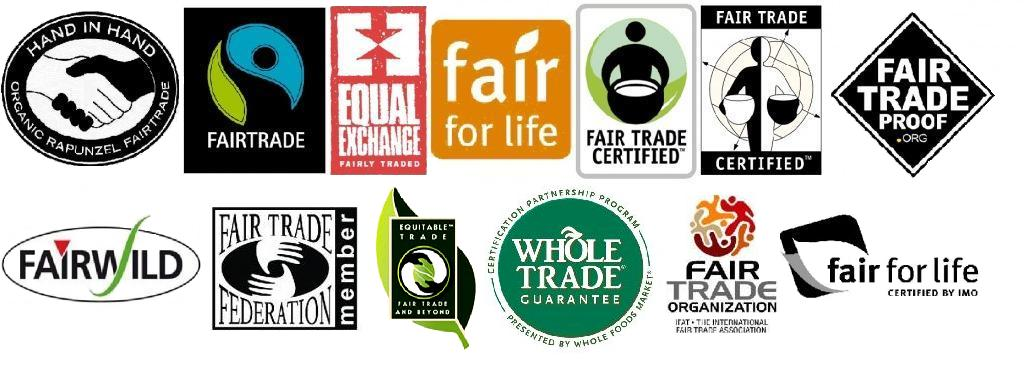
\includegraphics[width = \textwidth]{fair}


\includegraphics[trim =8cm 0 0 0, clip, width = 3cm]{fair2}
\end{frame}
% you are probalby familar examples of this is fair trade
% interestingly, FT US recently broke with FT international in order to srike a deal with walmart--an example of a "race to the bottom" thesis as FT us adjusted its regultory requirments in order to expand its marketshare



\begin{frame}
\frametitle{U.S. Forestry }
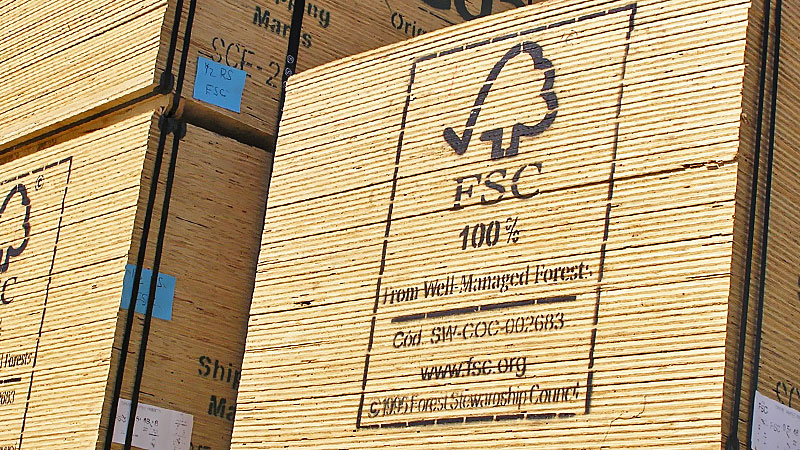
\includegraphics[width = \textwidth]{fscwood}
\end{frame}
% as private forestry regulations are the empirical case, i will use this case to illustrate 
% this scheme started in the early 90s when Greenpeace and the WWF and forest-dependent indigenous groups failed to get an international agreement on forest protection. The idea was that they would protect the amazon and indonesia, what actually happend is that these programs ended up having the most bite in the US, canada, and northern europe, where the companies are big, official, and care about their reputation



% activists targeted major consumer facing brands such as kleenex
\begin{frame}
\frametitle{Private Authority, Act 1: Protest}
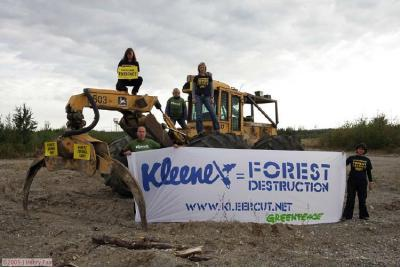
\includegraphics[width = \textwidth]{kleenex}

\end{frame}

% these tactics got the companies to capitulate 
\begin{frame}
\frametitle{Private Authority, Act 1: Protest}
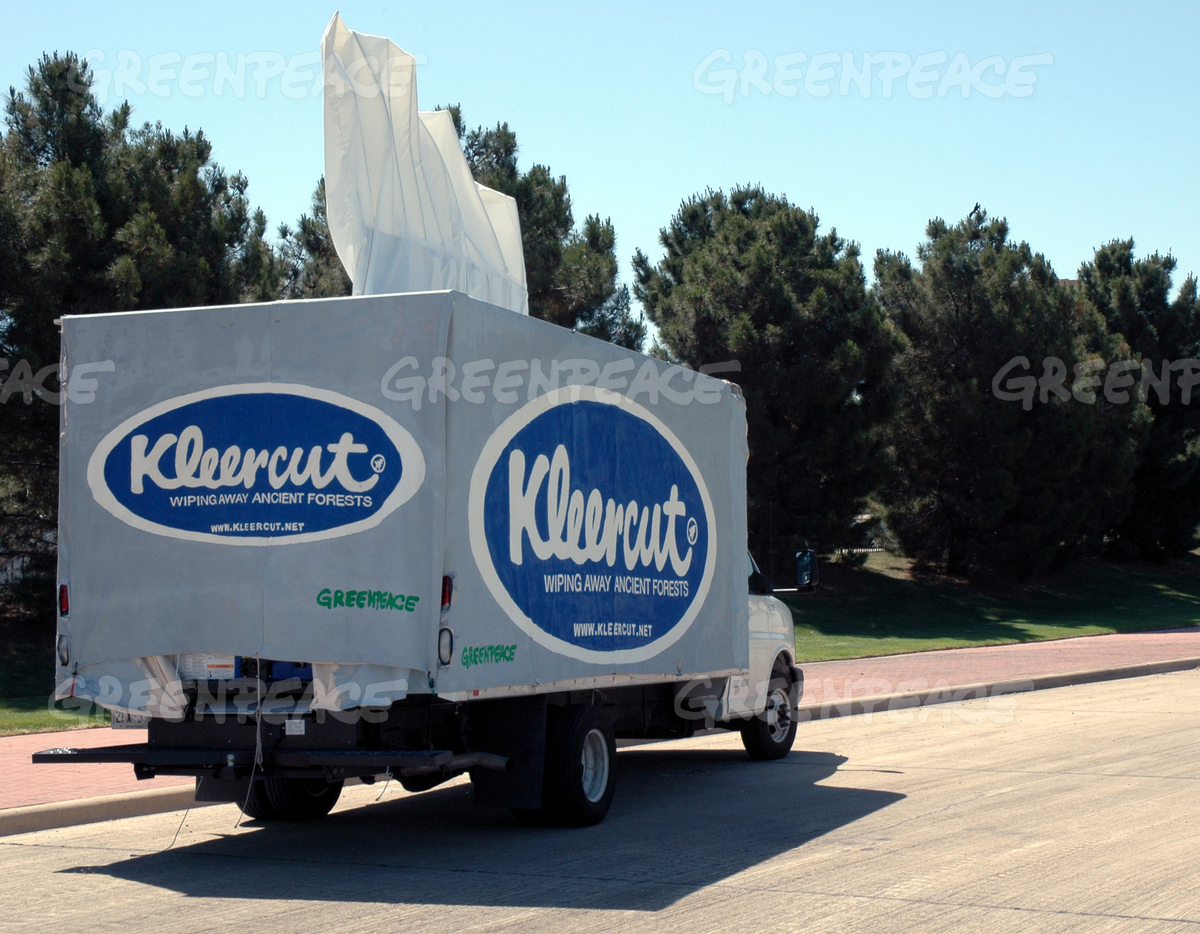
\includegraphics[width = \textwidth]{kleenex2}
\end{frame}

% when they did so, NGOs then lend their crediblity to the brand
\begin{frame}
\frametitle{Private Authority, Act 2: Demand}
\centering
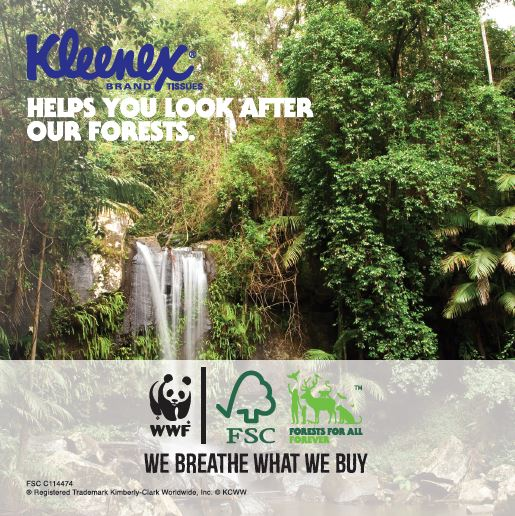
\includegraphics[height = \textheight]{kleenex3}
\end{frame}

% so if you buy anything at home depot
\begin{frame}
\frametitle{Private Authority, Act 2: Demand}
\centering

\includegraphics[height =7cm]{homedopot}
\end{frame}

% JK rowling insisted her books were printed on FSC certified paper
\begin{frame}
\frametitle{Private Authority, Act 2: Demand}
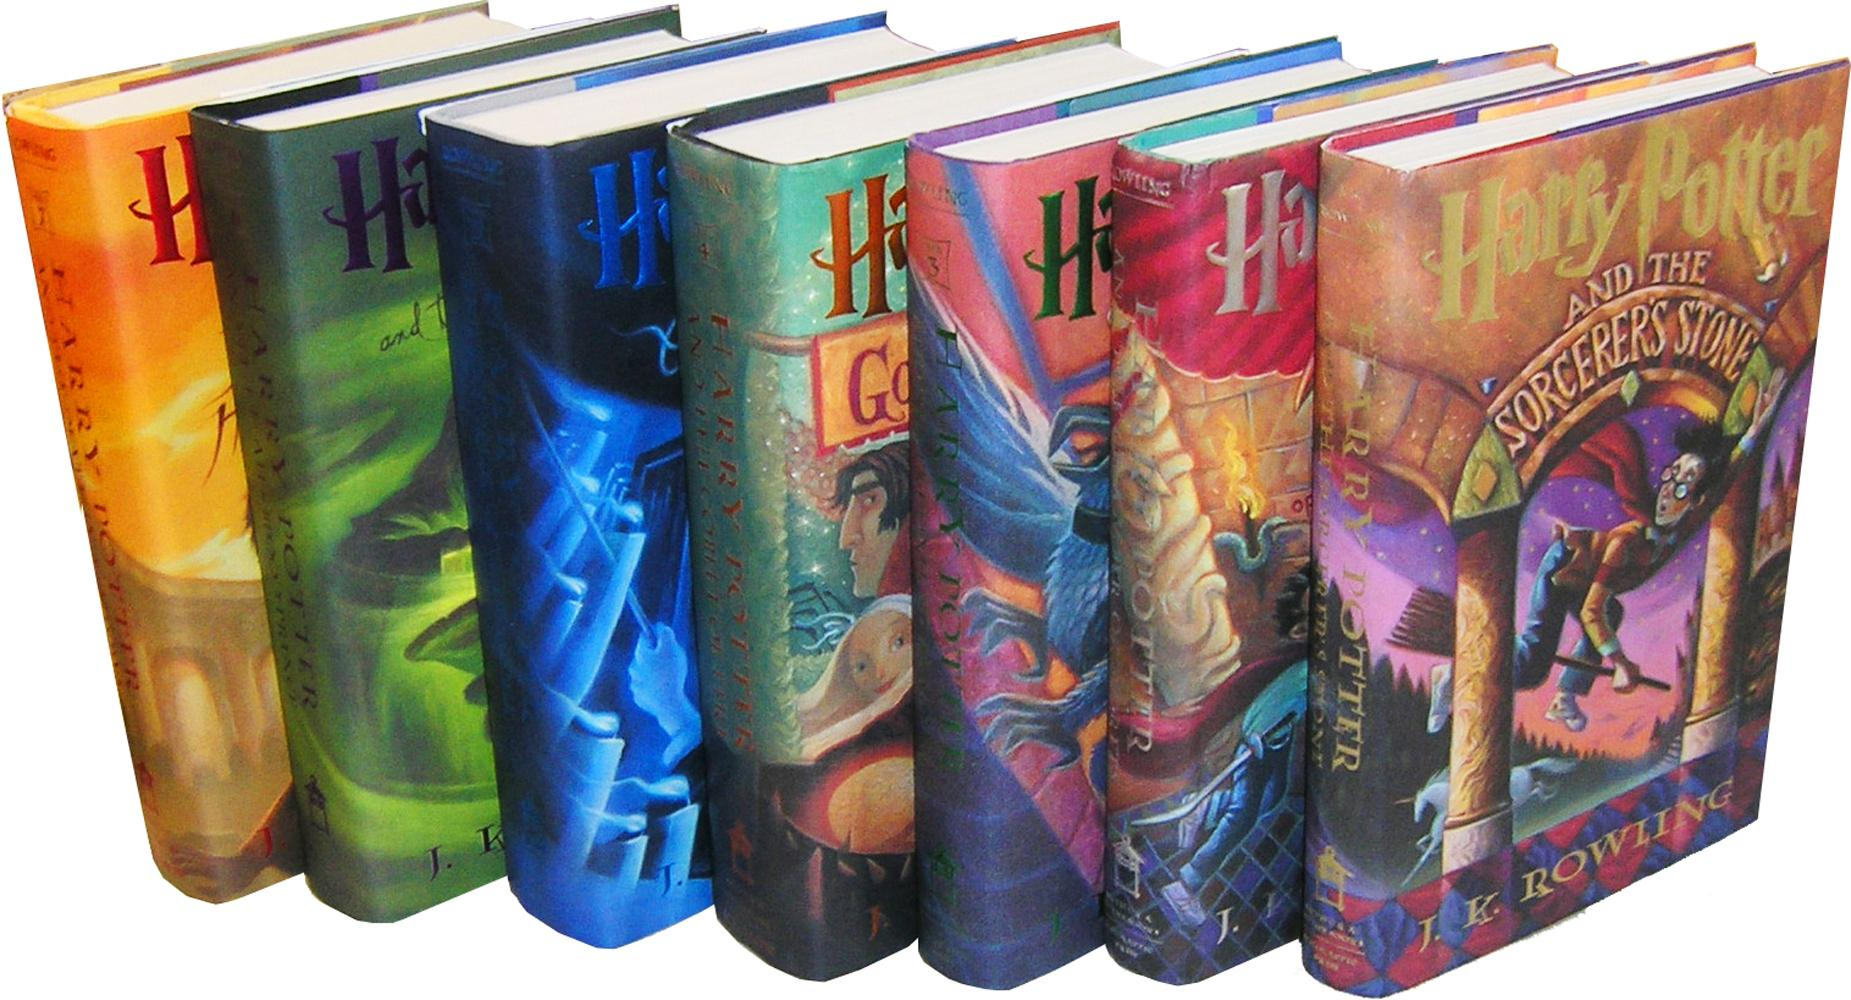
\includegraphics[width = \textwidth]{harrypotter}
\end{frame}

% it also includes presige brands like your APSR 
\begin{frame}
\frametitle{Private Authority, Act 2: Demand}

\includegraphics[width = \textwidth]{cambridge}
\end{frame}

% with all of these purchasing policies demanding compliant products gives programs like the FSC power over industry 
% in Wisconsin, the paper industry got the stat to pay for all of the paperwork and auditing to get pretty much all industrial forestry in the Wisconsin certified. 
\begin{frame}
\frametitle{Private Authority, Act 3: Supply}
\centering 
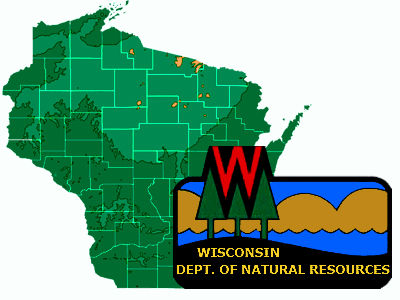
\includegraphics[width = 7cm]{dnr}

``Certification of forest management and chain of custody was pursued at the request of Wisconsin's paper industry as the industry was under the threat of losing major customers''
\end{frame}


% so that is one way NGOs like the FSC gain power. another is the way they garner legitimacy among key audiences. 
% THIS MAY DRIVE BYRON UP THE WALL, but here industry is the REDS and social activists are the YELLOWs
% as the FSC gained market share, the industry got unconmfortable and the American Forest and Paper Association started an alternative program and made all of their members participate in it. However, it lacked legitmacy, Home Depot when though a contentius process and decided not to accept it. In 1995 AFPA spun it of as its own NGO which started requireing third-party audits and a bunch of costly things; companeis still have majority of voting rights, but it is now actaully requiring things of them, no longer consensus greenwashing. 
\begin{frame}
\frametitle{Politics}

\includegraphics[width = 4cm]{fsclogo}   
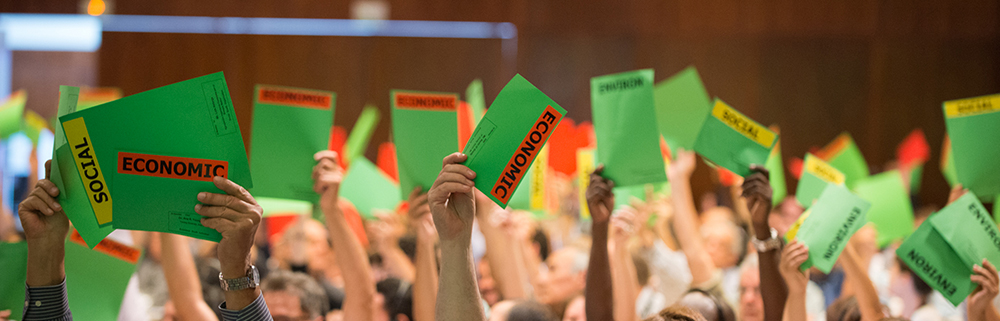
\includegraphics[width = 7cm]{fscvote} \pause

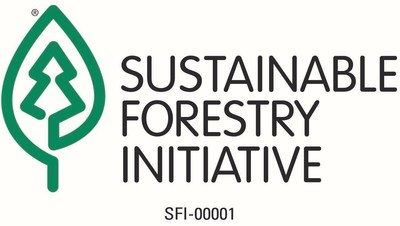
\includegraphics[width = 4cm]{sfilogo}   
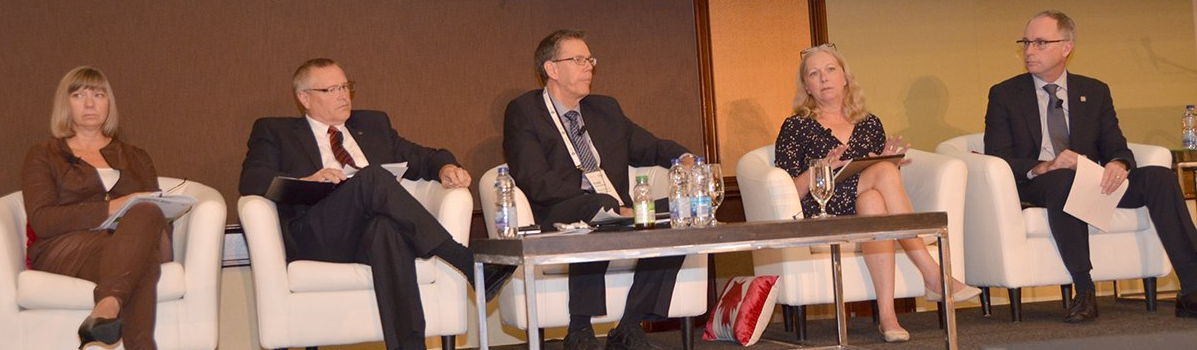
\includegraphics[width = 7cm]{sficon}
\end{frame}

% unlike fair trade, in US forestry, private authoirty truley regulates the industry, literally replacing the state in a nubmer of states where government inspectors don't even inspect certified forests because kwno they are being audidted for legal complinace and more. 
\begin{frame}
\begin{figure}[h!]
\centering
\caption{United States Timberland}
\label{acres}
\centering
\includegraphics[width=\textwidth]{acres2.pdf}
\centering
\footnotesize

%Sources: AF\&PA, 2016; PEFC, 2017; US Forest Service, 2009

%``Sustainable Forestry and Certification Programs in the United States'; US Forest Service (2009) ``Forest Resources of the United States''; PEFC (2017) ``Double certification on the rise,  joint PEFC/FSC data shows''
\end{figure}
\end{frame}


\section{Motivation}

% so what have scholars had to say about this? 
% a lot
% but these debates are in parte because no one is measuring the thing they are talkign about 
% most are just ipresionaistic, so cherry pick a few bits of evidence that supports their theory, and formal models just assuem proportional costs and benifits - more expensive is better - may be true, but does not tell us much 
% in the absene, sholars have assumed that who sponsors a program or public percemtiosn proxis for stringeny, which may also be true, but is exactly what everyone else is debating 
% there are also, orthoginal measures such as how many issues
\begin{frame}
\frametitle{Motivation}
Many theories of policy change
\begin{itemize}
\item ``race to the bottom'' (Gulbrandsen 2014)
\item ``converge'' toward ``higher'' standard (Overdevest and Zeitlen 2014)
\item converge to the middle bound by ``ceilings and floors'' (Cashore et al. 2004)
\item ``equilibrium'' (Fischer \& Lyon 2014) 
\item ``differentiation'' (Eberlein et al. 2014)
\end{itemize}\pause
Little measurement \pause
\begin{itemize}
\item high or low ``stringency'' \begin{itemize}
	\item unmeasured
    \item select issues 
    \item proportional cost and benefit (assumption) \pause
    \item perceived stringency (van der Ven 2015)
    \item backers (Darnall et al. 2010)
\end{itemize}
\item narrow or broad scope (Auld 2014, Heyes and Martin 2017)
\end{itemize}
\end{frame}

% and it is not just this narrow set of theories about whenther "races to the top of bottom" 
% all kinds of theories use policy content as a variable
% similar to public policy content, it .... 
\begin{frame}
\frametitle{The content of private regulations}
Like public policy: \begin{itemize}
  \item Impacting \begin{itemize}
    \item cost
    \item compliance rate
    \item outcomes \end{itemize} \pause
  \item Impacted by: \begin{itemize}
    \item balance of power among coalitions
    \item decision-making process 
    \item social and industry norms \end{itemize}
\end{itemize}

\end{frame}

% unlike, or at least to a different degree, it also 
\begin{frame}
\frametitle{The content of private regulations}
[Somewhat] unlike public policy: \begin{itemize}
	\item Impacting \begin{itemize}
      \item trust and legitimacy
      \item adoption by firms
      \item competitor response \end{itemize} \pause
	\item Impacted by \begin{itemize}
		\item market power/industry structure
        \item consumer behavior 
        \item activist and industry groups
	\end{itemize} \pause
    \item \textbf{Measured extremely poorly}
\end{itemize}
\end{frame}



\section{Concepts}

% so we try to focus scholars on a few diognostic questions about ends and means at different scales 
\begin{frame}
% table 2 questions
\begin{table}[h!]
\renewcommand{\arraystretch}{1.5} 
\centering
\caption{Measures of Policy Content}
\label{questions}
\end{table}
\centering
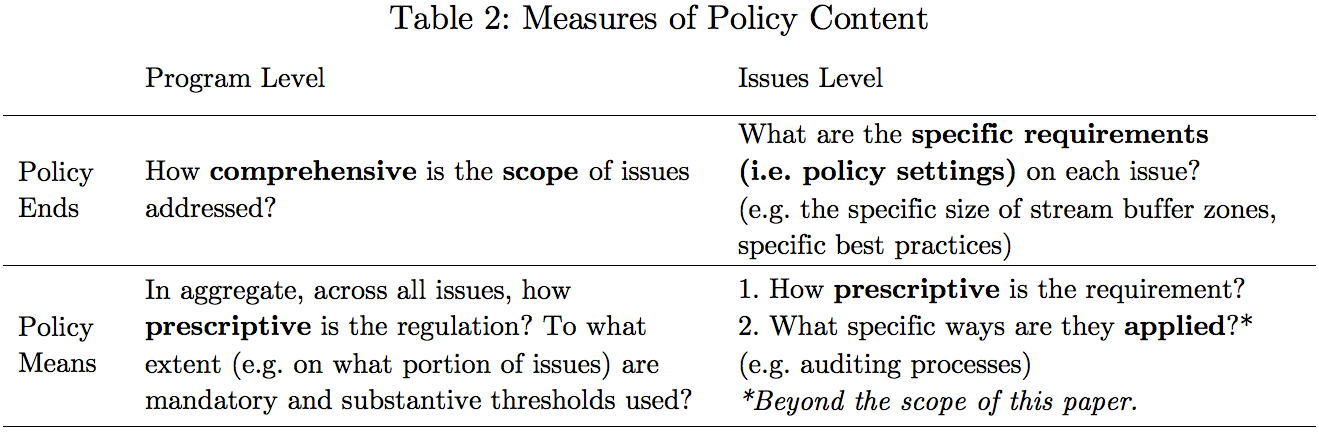
\includegraphics[trim=0 0 0 2.3cm,clip,width = \textwidth]{table2}
\end{frame}

% one key concept is the idea of how prescritpvive instruments are, how uch they are both mandadory and substantive, i.e. not suggestions and not just saying you need to make a plan/policy/proceedure
% in in a deeper sense, high and low are probaly the wrong way to be thinking about these things; high requiremnts aimed at protecting social values are very different than high requiremnts aimed at solving industry collective action problems, but hopefully the attention to comprehensiveness and disaggretion will call attention to those differences---.i.e that there are as many ways to answer the the high low question as there are overarching goals. 
\begin{frame}
% table 3 prescriptiveness 
\begin{table}[h!]
\footnotesize
\renewcommand{\arraystretch}{1.5} 
\centering
\caption{Prescriptiveness of policy  instruments}
\label{prescriptiveness}
\begin{tabular}{lccc}
 & \textbf{Discretionary} & \textbf{Non-discretionary} \\
 \cline{2-3} 
Procedural (plan- or systems-based) & Flexible & Somewhat prescriptive \\
 \cline{2-3} 
Substantive (e.g. a policy threshold) & Flexible & Most prescriptive \\
 \cline{2-3} 
\end{tabular}
\end{table}
\end{frame}

% that applies to lots of kinds of policy content, but those wanting to compare competing programs, will want to characterize there relationship over time, and we offer consistant terminology to do so
\begin{frame}
% table 4 patterns 
\begin{table}[h!]
\centering
\footnotesize
\renewcommand{\arraystretch}{1.2} 
\caption{Patterns of Change Among Private Regulations}
\label{patterns}
\begin{tabular}{cllll}
\multicolumn{1}{c}{}                                                                                  &                               & \multicolumn{3}{c}{}                                               \\ 
\multicolumn{1}{c}{}                                                                                  &                               & \multicolumn{3}{c}{\textbf{Relationship Among Standards}}                                               \\ 
\multicolumn{1}{c}{}                                                                                  & \multicolumn{1}{c}{}         & \multicolumn{1}{c}{Converging} & \multicolumn{1}{c}{Parallel} & \multicolumn{1}{c}{Diverging} \\ \cline{3-5} 
\multicolumn{1}{c}{\multirow{6}{*}{\begin{tabular}[c]{@{}c@{}}\textbf{Directions of Change} \\ (in comprehensiveness of scope, \\prescriptiveness of instruments, \\ \textit{or} levels of requirements)\end{tabular}}} & \multicolumn{1}{c|}{Increasing}   & \multicolumn{1}{c|}{\begin{rotate}{-30}$\nearrow$\end{rotate}}           & \multicolumn{1}{c|}{$\nearrow$}       & \multicolumn{1}{c|}{$\nearrow$}          \\
\multicolumn{1}{c}{} & \multicolumn{1}{l|}{}   & \multicolumn{1}{c|}{$\nearrow$}           & \multicolumn{1}{c|}{$\nearrow$}       & \multicolumn{1}{c|}{\begin{rotate}{-30}$\nearrow$\end{rotate}}          \\
\cline{3-5} 
\multicolumn{1}{c}{} & \multicolumn{1}{c|}{Opposite or }   & \multicolumn{1}{c|}{$\searrow$}           & \multicolumn{1}{c|}{$\longrightarrow$}       & \multicolumn{1}{c|}{$\nearrow$}          \\  
\multicolumn{1}{c}{} & \multicolumn{1}{c|}{Equilibrium}   & \multicolumn{1}{c|}{$\nearrow$}           & \multicolumn{1}{c|}{$\longrightarrow$}       & \multicolumn{1}{c|}{$\searrow$}          \\ \cline{3-5} 
\multicolumn{1}{c}{} & \multicolumn{1}{c|}{} & \multicolumn{1}{c|}{$\searrow$}           & \multicolumn{1}{c|}{$\searrow$}       & \multicolumn{1}{c|}{\begin{rotate}{30}$\searrow$\end{rotate}}          \\ 
\multicolumn{1}{c}{} & \multicolumn{1}{c|}{Decreasing} & \multicolumn{1}{c|}{\begin{rotate}{30}$\searrow$\end{rotate}}           & \multicolumn{1}{c|}{$\searrow$}       & \multicolumn{1}{c|}{$\searrow$}          \\ \cline{3-5} 
\end{tabular}
\end{table}
\end{frame}




% i am going to talk about the application briefly, but it was a huge task deeply in the weeds
% in short, we inductivly identified 48 issues that capture all of the things all of the standards deal with at a similar level of specifity. I then did a close legalistic textual analysis of their requiremnts on each. this was tricky becasue the SFI is written to sound like the FSC language, even using acronyms with the letters flipped. I coded them on their prescritpveness and nature of change. 
\section{Results}
\begin{frame}
\begin{figure}[h!]
\centering
\label{sfi}
\caption{Comparing FSC-US and SFI on Scope and Prescriptiveness}
\includegraphics[trim=0 0 0 9.3cm,clip, width=9.65cm]{FSCvSFItop.pdf}
\end{figure}
\end{frame}

% in sum, the scopes don't really change. SFI already matched FSC by haveing some requirements on most of their issues, and did not really change enough to match them. 
\begin{frame}
\begin{figure}[h!]
\centering
\label{sfi}
\caption{Comparing FSC-US and SFI on Scope and Prescriptiveness}
\includegraphics[trim=0 0 0 4.7cm,clip, width=9.65cm]{FSCvSFItop.pdf}
\end{figure}
\end{frame}


% prescipptiveness is a different story, nobody predicted that the more prescirptive regulation would get tougher since all of its external incentives seemed to dirve it downward. Overdivest who predicted SFI would go up, but assumed FSC was staying the same benchmark, it turns out the benchmark moved significantly. 
\begin{frame}
\begin{figure}[h!]
\centering
\label{sfi}
\caption{Comparing FSC-US and SFI on Scope and Prescriptiveness}
\includegraphics[trim=0 0 0 0cm,clip, width=9.65cm]{FSCvSFItop.pdf}
\end{figure}
\end{frame}


% now that we have a more clear idea what is going on, we are hoping to inspire future research into the causes. If this gets applied in other sectors, they may be able to pose similar questions. 
\begin{frame}
\frametitle{Future research: Why change?}
\begin{itemize}
	\item Organizational structure \begin{itemize}
      \item Restructuring constrained by core coalition
      \item Industry-backed program ``tying their hands?''
      \end{itemize} \pause
     \item Shifting market demand? \begin{itemize}
     	\item For one program?
        \item For certain requirements?
     \end{itemize} \pause
     \item Responding to decreasing trust and legitimacy? \pause
     \item ``Gradual transformation'' due to social norms/policy beliefs/goals 
\end{itemize}
\end{frame}

\begin{frame}
\frametitle{Thoughts?}
Literature and framing? 

\bigskip

Concepts of policy change?

\bigskip

Focusing causal research/theory?
\end{frame}










\end{document}

\begin{frame}
\begin{figure}[h!]
\centering
\label{pefc}
\caption{Comparing FSC-P\&C and PEFC on Scope and Prescriptiveness}
\includegraphics[width=\textwidth]{fig2pefc.pdf}
\end{figure}
\end{frame}

\begin{frame}
\begin{figure}[h!]
\centering
\label{sfi}
\caption{Comparing FSC-US and SFI on Scope and Prescriptiveness}
\includegraphics[width=\textwidth]{fig3sfi.pdf}
\end{figure}
\end{frame}
\end{document}